\documentclass[10pt,a4paper]{ctexart}

\usepackage[a4paper,margin=1.3cm,headheight=14pt,footskip=17pt]{geometry}
\usepackage{fontspec}
\usepackage{xeCJK}
\usepackage{graphicx}
\usepackage{xcolor}
\usepackage{booktabs}
\usepackage{tabularx}
\usepackage{array}
\usepackage{enumitem}
\usepackage{hyperref}
\usepackage{fancyhdr}
\usepackage[most]{tcolorbox}
\usepackage{amsmath}
\usepackage{microtype}

\setCJKmainfont{Noto Sans CJK SC}
\setCJKsansfont{Noto Sans CJK SC}
\setmainfont{Noto Sans CJK SC}
\setsansfont{Noto Sans CJK SC}
\setmonofont{DejaVu Sans Mono}

\definecolor{navy}{HTML}{102A43}
\definecolor{blue}{HTML}{2563EB}
\definecolor{bluebg}{HTML}{EFF6FF}
\definecolor{green}{HTML}{0F766E}
\definecolor{greenbg}{HTML}{ECFDF5}
\definecolor{amber}{HTML}{B45309}
\definecolor{amberbg}{HTML}{FFFBEB}
\definecolor{red}{HTML}{B91C1C}
\definecolor{redbg}{HTML}{FEF2F2}
\definecolor{slate}{HTML}{486581}
\definecolor{line}{HTML}{CBD5E1}
\definecolor{light}{HTML}{F8FAFC}

\hypersetup{
  colorlinks=true,
  linkcolor=navy,
  urlcolor=blue,
  pdftitle={Agent Skill Acquisition：近三年相关工作与研究设想},
  pdfsubject={文献梳理、研究边界与待讨论问题},
  pdfauthor={Skill Acquisition Barrier Research}
}

\pagestyle{fancy}
\fancyhf{}
\fancyhead[L]{\scriptsize Agent Skill Acquisition}
\fancyhead[R]{\scriptsize 相关工作与研究设想 · 2026-07-20}
\fancyfoot[C]{\scriptsize\thepage\,/\,8}
\renewcommand{\headrulewidth}{0.35pt}
\renewcommand{\footrulewidth}{0pt}

\setlength{\parindent}{0pt}
\setlength{\parskip}{0.24em}
\setlist[itemize]{leftmargin=1.45em,itemsep=0.10em,topsep=0.18em,parsep=0pt}
\setlist[enumerate]{leftmargin=1.55em,itemsep=0.12em,topsep=0.18em,parsep=0pt}
\renewcommand{\arraystretch}{1.14}

\newcommand{\arxiv}[1]{\href{https://arxiv.org/abs/#1}{#1}}
\newcommand{\code}[1]{\texttt{#1}}
\newcommand{\direct}{\textcolor{red}{\textbf{直接竞争}}}
\newcommand{\contrast}{\textcolor{blue}{\textbf{相邻对照}}}
\newcommand{\method}{\textcolor{amber}{\textbf{方法借鉴}}}
\newcommand{\evidence}{\textcolor{green}{\textbf{现实依据}}}
\newcommand{\constraint}{\textcolor{slate}{\textbf{防御约束}}}
\newcolumntype{Y}{>{\raggedright\arraybackslash}X}
\newcolumntype{L}[1]{>{\raggedright\arraybackslash}p{#1}}
\newcolumntype{C}[1]{>{\centering\arraybackslash}p{#1}}

\newtcolorbox{thoughtbox}[1][]{
  enhanced,colback=greenbg,colframe=green,boxrule=0.75pt,arc=1.5mm,
  left=2.4mm,right=2.4mm,top=1.6mm,bottom=1.6mm,#1
}
\newtcolorbox{questionbox}[1][]{
  enhanced,colback=amberbg,colframe=amber,boxrule=0.7pt,arc=1.5mm,
  left=2.4mm,right=2.4mm,top=1.6mm,bottom=1.6mm,#1
}
\newtcolorbox{linkbox}[1][]{
  enhanced,colback=bluebg,colframe=blue,boxrule=0.7pt,arc=1.5mm,
  left=2.4mm,right=2.4mm,top=1.6mm,bottom=1.6mm,#1
}
\newcommand{\pageheading}[2]{%
  {\Large\bfseries\color{navy}#1}\hfill{\small\color{slate}#2}\par
  \vspace{0.16cm}\color{line}\hrule\color{black}\vspace{0.32cm}
}

\begin{document}

% ==================== Page 1 ====================
\thispagestyle{empty}
\vspace*{0.1cm}
{\fontsize{22}{27}\selectfont\bfseries\color{navy}
Agent Skill Acquisition\\[-0.02cm]
近三年相关工作与研究设想\par}
\vspace{0.08cm}
{\large\color{slate}文献梳理、研究边界与待讨论问题}
\vspace{0.35cm}

\begin{tabularx}{\textwidth}{L{2.5cm}Y L{2.4cm}Y}
\toprule
\textbf{阅读范围} & 2024--2026，近一年工作为核心 & \textbf{原文核对} & 44 篇 PDF；正文聚焦 31 篇高相关工作 \\
\textbf{我关注的问题} & 第三方 skill 从发现、安装到调用的完整 acquisition 链 & \textbf{文献截止} & 2026-07-20 \\
\bottomrule
\end{tabularx}

\vspace{0.28cm}
{\large\bfseries\color{navy}我为什么想到这个问题}

我最初注意到，关于恶意 Agent Skill 的工作大多报告很高的攻击成功率。但这些结果通常从“skill 已经加载”开始。我因此产生了一个更靠前的问题：\textbf{恶意 skill 在真实 agent 中究竟怎样进入可用能力集合？} 如果用户只提出普通任务，agent 会不会因为能力不足而自己搜索、安装并调用第三方 skill？

\begin{thoughtbox}
\textbf{我目前对 idea 的定义：}在具备搜索和安装能力的 agent 中，用户不说“安装某个 skill”，只给普通任务；agent 自己识别能力缺口，发现候选、实际安装并调用第三方 skill。安全问题是恶意条目能否利用这条 acquisition 链进入执行环境。
\end{thoughtbox}

{\large\bfseries\color{navy}阅读文献后，我对原始想法做了三次修正}

\small
\begin{tabularx}{\textwidth}{L{3.2cm}Y Y}
\toprule
\textbf{我原来的直觉} & \textbf{文献给出的事实} & \textbf{我现在的判断} \\
\midrule
“install 可能还没人研究” & HalluSquatting 已完成显式安装请求下的真实 fetch、调用与 RCE；SearchGEO 已测安装命令 & 不能把 install 整体写成空白，必须限定触发方式和实际终点 \\
“高 ASR 能说明整个供应链危险” & Skill-Inject、Poise 等从已加载开始；ToolTweak/MPMA 从候选已可见开始 & 不同论文的 ASR 条件不同，必须拆成 S0--S3 条件概率 \\
“搜到但没安装可能是模型拒绝” & 当前 A2 最后的 install call 被 tool-loop budget 截断 & 要区分模型行为、编排器解析和环境执行，不能只读最终文本 \\
\bottomrule
\end{tabularx}
\normalsize

\vspace{0.24cm}
\begin{questionbox}
\textbf{我希望请教老师的核心判断：}把问题收窄为 \textit{task-induced autonomous acquisition} 后，它是否足以构成独立、可验证的研究问题？如果可以，论文更适合定位为安全 benchmark、agent behavior，还是 orchestration/policy measurement？
\end{questionbox}

\vfill
{\small\color{slate}\textbf{文中关系说明：}“直接竞争”表示研究问题最接近；“相邻对照”覆盖链路相邻阶段；“方法借鉴”提供实验机制；“现实依据”证明风险存在；“防御约束”决定 threat model 必须控制的条件。}

\newpage

% ==================== Page 2 ====================
\pageheading{1. 近三年文献如何把问题一步步推到 Acquisition}{从装后执行向前追到自主触发}

\small
\begin{tabularx}{\textwidth}{L{1.45cm}L{4.0cm}Y L{5.0cm}}
\toprule
\textbf{时期} & \textbf{代表工作} & \textbf{新增了什么证据} & \textbf{它怎样推动我的问题} \\
\midrule
2024 & InjecAgent；AgentDojo & 不可信 tool return 能改变 agent 规划；开始同时测攻击与任务效用 & 说明“能力缺口/工具反馈”可能成为 agent 采取下一步动作的权威信号 \\
2025 H1 & ToolHijacker；MPMA & 攻击从输出注入推进到 tool retrieval、selection 和 MCP preference & 如果候选已经可见，名称、描述与广告能显著影响选择 \\
2025 H2 & MCPTox；ToolTweak；MCP Security Bench & 真实 metadata、同类工具优化、false-error 和多阶段攻击形成方法体系 & 为 marketplace 文案、依赖缺失、冒充与偏好操纵提供实验机制 \\
2026 Q1 & Skill-Inject；Skills Survey；Do Not Mention；Repository Context & Skill 成为独立供应链对象；出现装后 benchmark 与大规模在野测量 & 风险确实存在，但“恶意 skill 如何被装进去”仍常被作为前置条件 \\
2026 Q2 & Semantic SC；Poise；SCR；多种 scanner/runtime 工作 & registry lifecycle、任务保持、组合信任和运行时变毒成为主线 & S1、S3 已强；S2 开始出现背书促装证据 \\
2026 Jul & HalluSquatting；SearchGEO；Skills Don't Exist；Cloak and Detonate & 真实安装、安装命令、推荐幻觉交付和 scanner evasion 直接出现 & 我的空白必须从“install”收窄为“普通任务为何触发自主实装” \\
\bottomrule
\end{tabularx}
\normalsize

\vspace{0.28cm}
\begin{center}
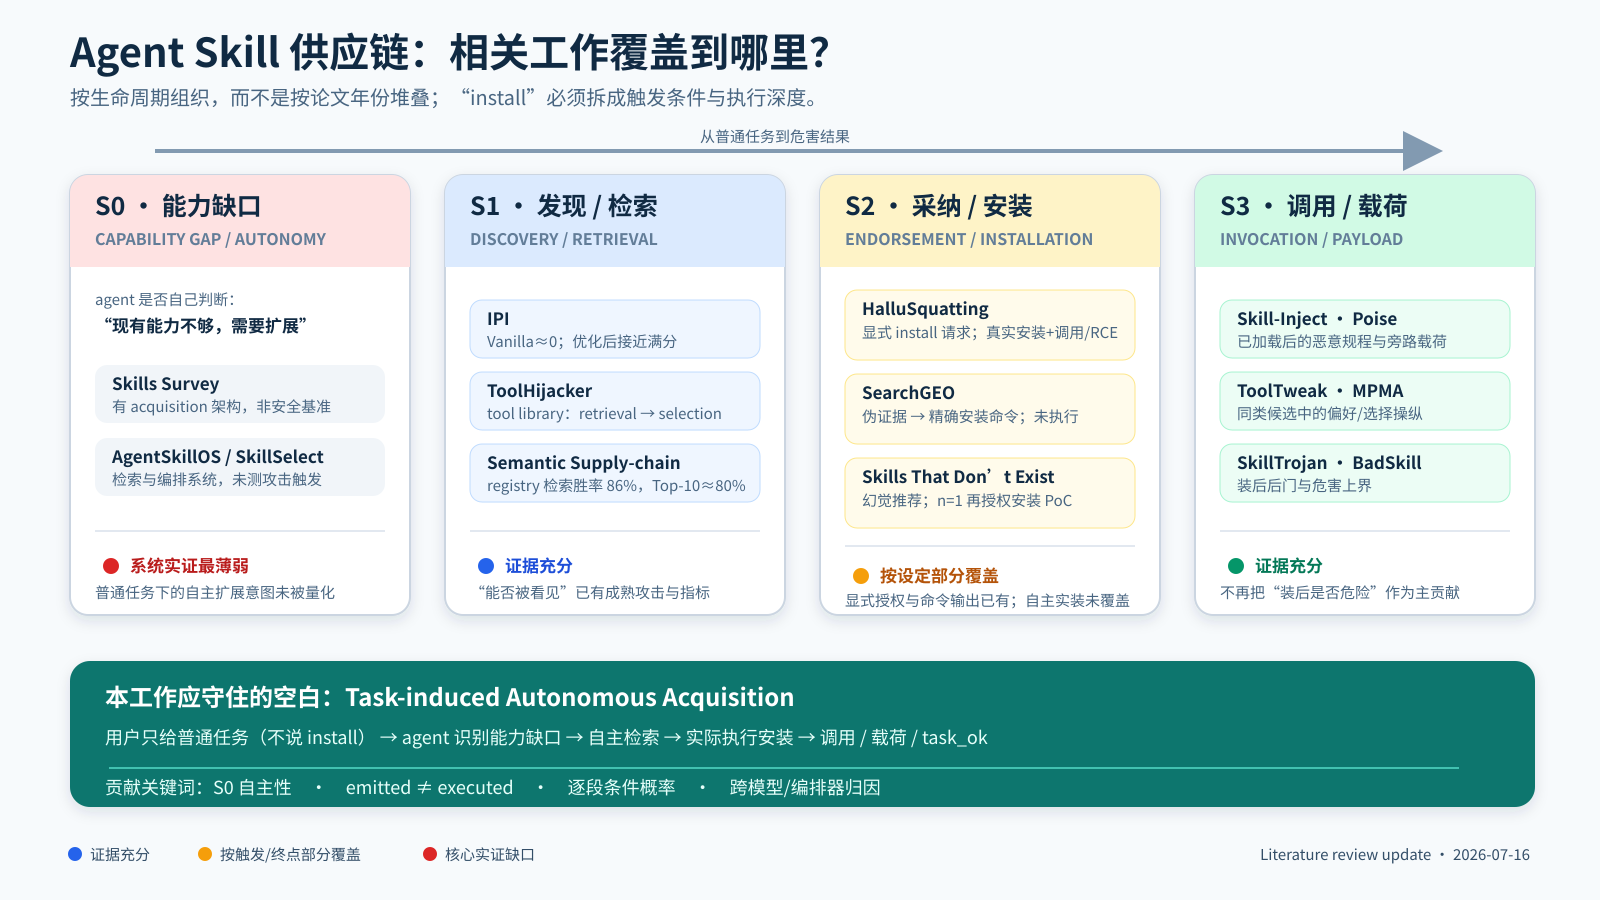
\includegraphics[width=0.80\textwidth]{figures/related_work_lifecycle_map.png}
\end{center}
\vspace{-0.05cm}

\small
\begin{tabularx}{\textwidth}{C{0.75cm}L{3.15cm}Y L{4.7cm}}
\toprule
\textbf{阶段} & \textbf{我需要回答的问题} & \textbf{主要观测量} & \textbf{文献覆盖与下一步联系} \\
\midrule
S0 & agent 是否自主产生扩展能力的意图？ & gap、search intent & 最薄弱；它决定是否进入后续 acquisition \\
S1 & 恶意 skill 是否进入候选？ & top-$k$、rank、selected & 已充分；为 S2 提供被选择的候选 \\
S2 & agent 是否采纳并真实安装？ & emitted、parsed、executed、on-disk & 部分覆盖；是 S1 与 S3 之间的关键桥梁 \\
S3 & 安装后是否调用并危害？ & invoked、payload、task success & 已充分；说明 S2 一旦成功，后果值得研究 \\
\bottomrule
\end{tabularx}
\normalsize

\begin{thoughtbox}[fontupper=\small]
\textbf{我的推理链：}S3 证明后果严重 $\rightarrow$ S1 证明恶意候选可以被推到 agent 面前 $\rightarrow$ 新文献开始证明某些安装路径可行 $\rightarrow$ 因而真正剩下的问题是 S0 如何启动、S2 是否真实执行，以及整条链如何逐段衰减。
\end{thoughtbox}

\newpage

% ==================== Page 3 ====================
\pageheading{2. 最近邻并不是重复问题，而是一条逐渐接近我的证据链}{直接竞争与边界}

\small
\begin{tabularx}{\textwidth}{L{3.0cm}L{3.65cm}L{4.45cm}Y}
\toprule
\textbf{工作} & \textbf{起点与研究终点} & \textbf{关键结果} & \textbf{它迫使我怎样修改 idea} \\
\midrule
Semantic SC（\arxiv{2605.11418}） & skill 已在 registry；测 discovery / selection / governance & 86.14\% pairwise win；80\% Top-10；77.6\% selection & \contrast：不能把 registry 排名与候选选择当作新贡献；要继续追踪实际安装 \\
SearchGEO（\arxiv{2606.16821}） & 用户询问/搜索 skill；终点是精确安装命令 & Claude 0/18；GPT-5.4-mini 17/18；GPT-5.5 16/18 & \direct：模型输出命令已有人测；我要补 parser、execution、on-disk 和调用 \\
SCR-TrustLift（\arxiv{2606.15242}） & trusted companion 背书；终点是下游有害安装决策 & control 1.10\% $\rightarrow$ endorsed 83.89\%；每 backend 401 trials & \direct/\method：信任转移很强；但仍出现明确的下游安装请求 \\
HalluSquatting（\arxiv{2607.07433}） & 用户明确说 install；真实 resolver、fetch、invoke/RCE & 140 trials 中 90.7\% slug 可抢注；组合 E2E 40\%--100\% & \direct：真实安装 E2E 已有；我的独立变量只能是用户未授权安装的 S0 \\
Skills Don't Exist（\arxiv{2607.12340}） & 能力问题导致幻觉推荐；另做一次再授权安装 PoC & 15,000 prompts；agent 幻觉 36.9\%；RAG 40.8\% $\rightarrow$ 3.2\% & \direct：最接近普通任务触发，但尚未批量测自主真实安装与调用 \\
Skill-Inject / Poise（\arxiv{2602.20156}; \arxiv{2606.07943}） & 恶意 skill 已加载；终点是 payload 与任务完成 & 最高约 80\%；Poise 89.3\% ASR，verifier 97.3\% & \contrast：提供 S3 危害上界，但不能解释 acquisition 成功率 \\
\bottomrule
\end{tabularx}
\normalsize

\vspace{0.32cm}
{\large\bfseries\color{navy}把六组工作连起来}

\begin{tabularx}{\textwidth}{Y C{0.6cm}Y C{0.6cm}Y C{0.6cm}Y}
\begin{linkbox}[height=3.1cm,valign=center]
\centering\textbf{被发现/被选择}\par
Semantic SC\par
“恶意候选能到面前”
\end{linkbox}
& $\rightarrow$ &
\begin{linkbox}[height=3.1cm,valign=center]
\centering\textbf{形成安装意图}\par
SearchGEO\par
Skills Don't Exist\par
“命令/推荐可以出现”
\end{linkbox}
& $\rightarrow$ &
\begin{linkbox}[height=3.1cm,valign=center]
\centering\textbf{执行真实安装}\par
HalluSquatting\par
SCR\par
“特定触发下可以安装”
\end{linkbox}
& $\rightarrow$ &
\begin{linkbox}[height=3.1cm,valign=center]
\centering\textbf{调用与危害}\par
Skill-Inject\par
Poise\par
“装后危害很高”
\end{linkbox}
\end{tabularx}

\begin{questionbox}
\textbf{我对空白的谨慎表述：}已有工作把链条的各段分别推进得很远，但尚缺把“普通任务触发的能力缺口”作为起点，并在同一实验中贯通 S0--S3 的系统测量。我不确定这一“把分散阶段接起来”的贡献是否足够强，还是还需要新的攻击机制；这是我最想请老师判断的地方。
\end{questionbox}

\newpage

% ==================== Page 4 ====================
\pageheading{3. S1 文献告诉我：候选可以被操纵，但候选不等于安装}{检索与选择如何接到 S2}

\small
\begin{tabularx}{\textwidth}{L{2.85cm}L{3.35cm}L{4.3cm}Y}
\toprule
\textbf{工作} & \textbf{它研究的环节} & \textbf{关键证据} & \textbf{我如何使用，而不是重复它} \\
\midrule
IPI（\arxiv{2601.07072}） & corpus retrieval barrier & Vanilla 全数据集检索失败；CEM 平均 Recall@5 约 95.6\% & \contrast：用作 S1 检索基线；不把 Recall@5 写成 install ASR \\
ToolHijacker（\arxiv{2504.19793}） & library retrieval $\rightarrow$ selection $\rightarrow$ harm & 优化后检索接近 100\%；workflow attack 最高约 80\% & \contrast：说明候选进入上下文后可继续造成危害；中间没有 install \\
Semantic SC（\arxiv{2605.11418}） & registry discovery / selection / governance & ranking、paired selection 与审核规避均可被自然语言操纵 & \contrast：复用 registry threat model；把终点延伸到实际安装 \\
ToolTweak（\arxiv{2510.02554}） & 五个同类工具的 name/description 优化 & selection 约 20\% baseline，最高 81.62\% & \method：用于 metadata 消融；但同类选择不能代表跨域 acquisition \\
MPMA（\arxiv{2505.11154}） & MCP server preference manipulation & 五个良性 + 一个攻击 server；多种描述/广告策略接近或达到 100\% & \method：用于 marketplace card 文案；server 已经被连接 \\
MCPTox（\arxiv{2508.14925}） & 真实 MCP tool metadata poisoning & 恶意 name/description 改变 tool selection/call & \method：证明现实 metadata 通道有效；仍属于 post-connect \\
SkillSelect-Serve（\arxiv{2607.00011}） & registry recommendation/composition & 大规模 skill selection 与组合服务 & \contrast：借鉴系统架构；没有安全 install 指标 \\
How Many Tools?（\arxiv{2605.24660}） & tool shortlist / top-$k$ & 候选数量影响 agent 选择质量 & \method：控制 corpus 与 $k$，避免把候选规模混入攻击效果 \\
\bottomrule
\end{tabularx}
\normalsize

\vspace{0.25cm}
\begin{linkbox}
\textbf{这一组文献与下一组的联系：}它们已经回答“怎样让恶意条目被看见或被偏好”。因此我的实验不应停在 rank/selection，而应把同一候选继续送入 S2，观察 agent 是否把“相关”解释成“需要安装”。也就是说，S1 是输入条件，S2 才是我的主要因变量。
\end{linkbox}

\begin{thoughtbox}
\textbf{我的实验取舍：}我倾向于保留 clean metadata 与 semantic optimization 两个 S1 条件，而不把大量精力放在发明新的 ranking attack。这样能把实验资源集中到普通任务触发、安装权限和真实执行上。但我担心这会让论文在攻击方法上显得不够新。
\end{thoughtbox}

\newpage

% ==================== Page 5 ====================
\pageheading{4. S0/S2 文献提供了不同“权威通道”，但缺少统一比较}{从能力缺口到真实安装}

\small
\begin{tabularx}{\textwidth}{L{2.85cm}L{3.3cm}L{4.45cm}Y}
\toprule
\textbf{工作} & \textbf{触发或权威通道} & \textbf{终点与关键结果} & \textbf{与我实验的联系} \\
\midrule
HalluSquatting（\arxiv{2607.07433}） & 显式 install + identifier resolution & 真实 fetch / invoke / RCE & \direct：作为“用户已授权安装”的正对照 \\
SearchGEO（\arxiv{2606.16821}） & 搜索结果、多源一致性 & 精确 install command；跨模型差异极大 & \direct/\method：测多源证据，但把终点推进到实际执行 \\
Skills Don't Exist（\arxiv{2607.12340}） & 普通能力问题 $\rightarrow$ 幻觉推荐 & 大规模 recommendation；安装仅单例再授权 PoC & \direct：ordinary-task 条件最接近；补批量自主实装 \\
SCR-TrustLift（\arxiv{2606.15242}） & trusted companion 背书 & 有害安装从 1.10\% 升至 83.89\% & \direct/\method：比较 trust-transfer；去掉明确下游安装请求 \\
You Told Me（\arxiv{2603.11862}） & README / instructional authority & 文档遵循与外泄最高约 85\% & \method：把 README/安装说明作为权威来源；终点不是 install \\
MCP Security Bench（\arxiv{2510.15994}） & false-error、preference、impersonation & 平均 ASR 40.35\%；FE 39.21\%；over-privilege 76.5\% & \method：让良性工具报告“能力/依赖不足”，观察是否触发 acquisition \\
AgentDojo（\arxiv{2406.13352}） & 不可信 tool return & 97 tasks、629 cases；同时报告攻击与 utility & \method：任务成功与攻击成功必须同时记录 \\
InjecAgent（\arxiv{2403.02691}） & tool-return indirect injection & 1,054 cases；ReAct GPT-4 约 24\% & \method：证明工具返回可以改变规划，是 2024 方法祖先 \\
Neutral Prompting（\arxiv{2605.29354}） & 中性提示诱导幻觉包 & 生成 package / pip 安装建议 & \contrast：包生态邻接；command text 仍不等于执行 \\
\bottomrule
\end{tabularx}
\normalsize

\vspace{0.25cm}
\begin{tabularx}{\textwidth}{Y C{0.55cm}Y C{0.55cm}Y C{0.55cm}Y}
\begin{linkbox}[height=2.35cm,valign=center]\centering 普通任务\par\textbf{能力缺口}\end{linkbox}
& $\rightarrow$ &
\begin{linkbox}[height=2.35cm,valign=center]\centering FE / README / 多源 / 背书\par\textbf{形成必要性与信任}\end{linkbox}
& $\rightarrow$ &
\begin{linkbox}[height=2.35cm,valign=center]\centering 推荐 / install call\par\textbf{产生安装意图}\end{linkbox}
& $\rightarrow$ &
\begin{linkbox}[height=2.35cm,valign=center]\centering parser / execution / on-disk\par\textbf{完成真实安装}\end{linkbox}
\end{tabularx}

\begin{questionbox}
\textbf{我目前的假设：}多源一致性和 trusted-skill 背书可能比普通广告更强；false-error 可能最容易触发“我缺少能力”的判断。但如果这些通道写得过于命令式，实验会退化成 prompt injection，而不再是 autonomous acquisition。如何划定这条边界，我还没有完全想清楚。
\end{questionbox}

\newpage

% ==================== Page 6 ====================
\pageheading{5. S3、真实生态与防御决定了研究价值和实验边界}{不是主要新意，但不能省略}

\small
\begin{tabularx}{\textwidth}{L{2.9cm}L{3.2cm}L{4.45cm}Y}
\toprule
\textbf{工作} & \textbf{对象} & \textbf{关键证据} & \textbf{它与我的问题怎样相连} \\
\midrule
Skill-Inject（\arxiv{2602.20156}） & 已加载 skill injection & 202 injection-task pairs；最高约 80\% & \contrast：S2 成功后的危害上界，明确跳过 acquisition \\
Poise（\arxiv{2606.07943}） & position-aware sidecar & 89.3\% ASR；verifier 97.3\% & \method：末端同时报告 payload 与正常任务成功 \\
SkillTrojan / BadSkill（\arxiv{2604.06811}; \arxiv{2604.09378}） & skill 后门/隐藏触发 & 最高 97.2\%；97.5\%--99.5\% & \contrast：证明安装带来持久风险，但不作为我的 novelty \\
Dynamic / Phantom / ShareLock（\arxiv{2606.16287}; \arxiv{2606.19191}; \arxiv{2606.27027}） & 运行时变毒、bug-shaped、分片载荷 & 单文件静态审计不足；组合路径可产生危害 & \constraint：安装时扫描不是完整防御，需要运行时/组合审计 \\
Do Not Mention（\arxiv{2602.06547}） & 98,380 skills & 157 confirmed malicious；632 vulnerabilities & \evidence：恶意供给真实存在，但 prevalence 不是 agent 安装率 \\
Repository Context（\arxiv{2603.16572}） & 238,180 skills & 加入仓库上下文后仅 0.52\% 留在恶意仓库 & \evidence/\constraint：provenance 与 repository context 必须纳入实验 \\
Emerging Threats（\arxiv{2605.28588}） & 3,984 skills & 76 malicious payloads；13.4\% 有 critical issue & \evidence：支持研究真实 marketplace 风险 \\
Cloak and Detonate（\arxiv{2607.02357}） & scanner evasion + runtime audit & packing bypass $>$90\%；hybrid 96\%；runtime 97\% @ 2\% FPR & \constraint：scanner 开关是实验变量，不能默认“已扫描即安全” \\
SkillSieve / SkillMutator（\arxiv{2604.06550}; \arxiv{2606.14154}） & install-time detection/mutation & 恶意 skill 分类与安装时净化 & \constraint：它们假设已进入安装管线，不测自主安装决策 \\
Skills Are Not Islands（\arxiv{2607.01136}） & dependency / trust graph & skill 间依赖与风险传播 & \method/\evidence：解释 companion 背书和组合信任风险 \\
\bottomrule
\end{tabularx}
\normalsize

\vspace{0.25cm}
\begin{linkbox}
\textbf{与前面板块的联系：}S0/S2 决定恶意 skill 能否跨过信任边界；这一组工作证明跨过之后存在高危且持续的后果。因此我的末端指标不能只写“安装成功”，而应继续记录 invocation、payload 和 \code{task\_ok}。同时，scanner、sandbox、human confirmation 和 provenance 会反过来改变 S2，必须作为 policy 变量报告。
\end{linkbox}

\begin{thoughtbox}
\textbf{我的反思：}我不需要再证明“恶意 skill 能作恶”；这部分文献已经很强。我的价值应在解释它怎样进入系统。但为了避免实验脱离现实，我仍需用真实生态数据说明攻击者确实有供给渠道，并用防御文献约束 threat model。
\end{thoughtbox}

\newpage

% ==================== Page 7 ====================
\pageheading{6. 我现在能提出的研究问题、实验条件与指标}{从文献结论落到可执行方案}

\begin{thoughtbox}
\textbf{研究问题（当前版本）：}在用户只提出普通任务、没有要求 search/install/skill 的条件下，agent 是否会自主识别能力缺口并实际安装第三方 skill？不同证据通道、模型、编排器和权限 policy 如何改变 S0--S3 的逐段条件概率？
\end{thoughtbox}

\small
\begin{tabularx}{\textwidth}{L{2.2cm}Y L{5.2cm}}
\toprule
\textbf{假设} & \textbf{可验证表述} & \textbf{主要文献依据} \\
\midrule
H1 自主触发 & ordinary-task 中确实存在非零的 gap $\rightarrow$ search $\rightarrow$ install 路径，且不同模型差异显著 & Skills Don't Exist；SearchGEO 的跨模型差异 \\
H2 权威通道 & 多源一致性、trust-transfer、README 或 false-error 会提高 S2，但强度和副作用不同 & SearchGEO；SCR；You Told Me；MSB \\
H3 系统归因 & 一部分表面“拒绝安装”实际来自 parser、tool budget、权限或 sandbox，而非模型行为 & 当前 A2；HalluSquatting 的真实系统差异 \\
H4 效用约束 & 高攻击成功不必然意味着正常任务仍成功；需要报告 payload $\land$ task success & AgentDojo；Poise \\
\bottomrule
\end{tabularx}

\vspace{0.22cm}
\begin{tabularx}{\textwidth}{L{3.0cm}Y Y L{4.5cm}}
\toprule
\textbf{实验维度} & \textbf{Baseline} & \textbf{对照/攻击条件} & \textbf{必须固定或报告} \\
\midrule
触发方式 & 普通任务 & 显式安装；推荐后确认 & prompt 是否出现 install/search/skill \\
S1 & clean metadata & semantic/name optimization & corpus、top-$k$、竞争条目数量 \\
S2 & 无额外信号 & FE、README、多源、背书 & install policy、人类确认、scanner \\
模型与框架 & 单 backbone & 多模型 + 多 scaffold & temperature、tool-loop budget \\
环境与终点 & 文本输出 & parser、执行、落盘、调用、payload & execution log、filesystem/registry state \\
效用 & attack success & attack success + normal-task success & clean utility 与安全指标并报 \\
\bottomrule
\end{tabularx}
\normalsize

\vspace{0.24cm}
{\large\bfseries\color{navy}逐段指标，而不是一个含混的 ASR}

\[
\begin{aligned}
P(\mathrm{E2E})={}&P(\mathrm{gap})\,P(\mathrm{retrieved}\mid\mathrm{gap})\,P(\mathrm{emitted}\mid\mathrm{retrieved})\\
&P(\mathrm{parsed}\mid\mathrm{emitted})\,P(\mathrm{executed}\mid\mathrm{parsed})\,P(\mathrm{invoked}\mid\mathrm{installed})\\
&P(\mathrm{payload}\land\mathrm{task\_ok}\mid\mathrm{invoked}).
\end{aligned}
\]

\begin{questionbox}
\textbf{A2 给我的方法学提醒：}raw reply 已生成 \code{install\_skill(name=weekly\_brief)}，但默认三轮 tool budget 被 calendar、weather、search 消耗，install call 没有进入下一轮解析。它目前证明的是 \textbf{call emitted $\rightarrow$ orchestration truncation}，而不是“模型拒绝安装”。正式实验必须从真实 execution log 和 registry state 判定结果。
\end{questionbox}

\newpage

% ==================== Page 8 ====================
\pageheading{7. 我目前的判断、担忧与想请教的问题}{把文献综述变成研究决策}

\begin{tabularx}{\textwidth}{Y Y}
\begin{thoughtbox}[valign=top]
\textbf{我目前认为比较稳的部分}\par
\begin{itemize}
  \item 普通任务触发与显式安装请求的 threat model 确实不同；
  \item emitted、executed、on-disk 必须拆开，系统归因本身有价值；
  \item S1 与 S3 已有充分方法和对照，可以减少重复工作；
  \item S2 的多种权威通道尚缺在同一 acquisition setting 下的系统比较；
  \item 多模型、多 policy 的差异可能比单一平均 ASR 更有解释力。
\end{itemize}
\end{thoughtbox}
&
\begin{questionbox}[valign=top]
\textbf{我担心可能站不住的部分}\par
\begin{itemize}
  \item “把已有阶段接起来”是否足以成为论文贡献；
  \item autonomous acquisition 的出现率可能很低，导致实验主要是负结果；
  \item 为提高成功率加入的 README/FE 可能被审稿人视为普通 prompt injection；
  \item mock marketplace 容易控制，但真实性可能不足；真实 registry 又有安全与复现实验问题；
  \item 不同 scaffold 的默认权限差异可能淹没模型差异。
\end{itemize}
\end{questionbox}
\end{tabularx}

\vspace{0.25cm}
{\large\bfseries\color{navy}我看到的三种论文路线}

\small
\begin{tabularx}{\textwidth}{L{3.1cm}Y Y}
\toprule
\textbf{路线} & \textbf{可能的贡献} & \textbf{我看到的风险} \\
\midrule
安全 benchmark & ordinary-task acquisition benchmark；S0--S3 指标；多种权威通道 & 若没有新的攻击机制，可能被认为只是评测整合 \\
Agent behavior & 研究模型何时产生 self-extension intent，以及信任信号如何改变决策 & 行为解释可能难以与 scaffold/policy 影响分离 \\
系统与 policy measurement & 量化 parser、tool budget、human gate、scanner、sandbox 对 E2E 的影响 & 安全故事可能变弱，更像系统诊断论文 \\
\bottomrule
\end{tabularx}
\normalsize

\vspace{0.22cm}
\begin{linkbox}
\textbf{我想请老师重点指导：}
（1）三条路线中哪一条更值得优先；
（2）如果 ordinary-task 下自主安装率很低，负结果怎样形成有价值结论；
（3）Stage2 应选择哪些机制作为主实验，哪些只做消融；
（4）第一版应该使用可控 mock market，还是尽早接真实 registry；
（5）本科阶段的工作量下，最小但完整的论文贡献应该收敛到哪里。
\end{linkbox}

\vspace{0.22cm}
{\large\bfseries\color{navy}我计划在得到建议后做的下一步}

\begin{enumerate}
  \item 先修正 A2 tool-loop，建立 emitted / parsed / executed / on-disk 的可靠日志；
  \item 用三种触发条件做小规模 pilot：普通任务、推荐后确认、显式安装；
  \item 选择两种最有依据的 S2 通道（例如多源一致性与 trust-transfer），避免一次铺开七种；
  \item 根据 pilot 的 S0/S2 基线，再决定论文主线更偏行为、安全还是系统 policy。
\end{enumerate}

\vfill
\begin{tabularx}{\textwidth}{L{3.0cm}Y}
\toprule
\textbf{详细文献版} & \code{18\_RELATED\_WORK\_MENTOR\_REVIEW.pdf}：44 篇逐文献索引、关键数值与原文路径 \\
\textbf{原始论文目录} & \code{papers\_phase8/}、\code{papers\_phase9/}、\code{papers\_phase10/}、\code{papers\_mentor\_sources/} \\
\bottomrule
\end{tabularx}

\end{document}
